\section{Problem and data description}
\subsection{Motivation and scope of this draft}
Underwater debris is difficult to distinguish from marine life and the seafloor because object appearance, scale, illumination and occlusion vary. TrashCan supplies underwater images with object-level annotations for marine debris research\cite{trashcan}. This project converts the polygons into a semantic segmentation task: each valid image pixel receives one class label, without distinguishing separate instances of the same class.

For an RGB image $x\in\mathbb{R}^{H\times W\times 3}$, the model predicts a map $\hat y\in\{0,\ldots,16\}^{H\times W}$. There are \textbf{17 output classes: background plus 16 foreground categories}. The foreground comprises ROV, plant, six animal categories and eight trash categories. Ignore label 255 is excluded from supervision and evaluation.

The research question is whether a pretrained modern segmentation model and modest photometric augmentation improve foreground overlap under a split that separates videos. This M2 draft reports the work completed through 28 October 2026: a completed U-Net experiment, an incomplete S0 SegFormer main run, and successful S0/S1 GPU pilots. It separates those observations from the remaining controlled comparison.

\subsection{Dataset source and provenance}
The working dataset is TrashCan 1.0 Material. The exploratory data analysis (EDA), measured on 5 October 2026, records 7,212 RGB images,12,336 polygon annotations and 312 filename-derived video groups. There are 3,245 images at $480\times 360$ and 3,967 at $480\times 270$. Source imagery is credited to JAMSTEC and the dataset to Hong, Fulton and Sattar\cite{trashcan}.

The source archive's license file and the annotation JSON license records are retained with the project evidence. The JSON records identify an Attribution-NonCommercial-ShareAlike entry; the archive also contains its own attribution and use statement. The report preserves both records rather than replacing them with an inferred license. Raw images, checkpoints and the large dataset archive are not redistributed in the report source package.

The instructor approved the proposal according to the project owner's confirmation on 26 October 2026. This statement records the confirmation used by the training setup; it is not an independently inspected learning-management-system submission record.

\subsection{Video-disjoint partition and class support}
The original source partitions contain 6,008 training images and 1,204 validation images. They share 127 filename-derived video IDs. Separating individual frames using those source labels would therefore allow frames from the same video into different evaluation partitions.

The project instead uses a fixed seed 36 manifest that assigns each video to exactly one partition. Metadata-based split construction uses deterministic greedy/local-search candidates, with at least three supporting training videos and two supporting videos in each held-out partition per foreground class. Table~\ref{tab:split} records the resulting image, video and annotation counts. Pairwise video-ID overlap is zero.
\begin{table}[H]
\centering\small
\caption{Fixed video-disjoint partition, split seed 36. Native mask percentages are retained from the 5 October 2026 EDA.}\label{tab:split}
\begin{tabular}{lrrrrr}\toprule
Partition & Images & Videos & Annotations & Background (\%) & Ignore (\%) \\ \midrule
Train & 5,057 & 207 & 8,563 & 89.13 & 0.0371 \\
Validation & 1,077 & 54 & 1,956 & 89.34 & 0.0754 \\
Test & 1,078 & 51 & 1,817 & 90.33 & 0.0238 \\
\bottomrule\end{tabular}
\end{table}

Video grouping addresses frame-level overlap under the chosen ID convention. It does not prove independence of dive locations or visually related scenes carrying different video IDs.

Class imbalance remains substantial after splitting. Table~\ref{tab:support} gives each foreground class's annotation count, video support and native supervised pixel totals. The small support for categories such as animal shells makes macro overlap and per-class results more informative than background-dominated accuracy.
\begin{table}[H]
\centering\small
\caption{Foreground class support in the fixed split. Pixel counts are native-resolution supervised pixels in millions, before letterboxing.}\label{tab:support}
\begin{tabular}{lrrrrrrr}\toprule
Class & Ann. & \multicolumn{3}{c}{Videos (train/val/test)} & \multicolumn{3}{c}{Pixels, M (train/val/test)} \\ \midrule
\cls{rov} & 3317 & 99 & 22 & 24 & 39.554 & 7.164 & 6.736 \\
\cls{plant} & 507 & 17 & 10 & 5 & 2.363 & 0.586 & 0.661 \\
\cls{animal_fish} & 764 & 33 & 7 & 5 & 4.421 & 1.444 & 1.577 \\
\cls{animal_starfish} & 398 & 9 & 3 & 3 & 0.123 & 0.037 & 0.022 \\
\cls{animal_shells} & 249 & 3 & 2 & 2 & 0.104 & 0.087 & 0.006 \\
\cls{animal_crab} & 309 & 9 & 3 & 3 & 0.789 & 0.199 & 0.196 \\
\cls{animal_eel} & 343 & 24 & 6 & 5 & 0.255 & 0.057 & 0.076 \\
\cls{animal_etc} & 235 & 12 & 6 & 7 & 0.805 & 0.079 & 0.177 \\
\cls{trash_etc} & 2039 & 107 & 23 & 23 & 9.145 & 1.921 & 1.601 \\
\cls{trash_fabric} & 314 & 14 & 4 & 3 & 2.285 & 0.422 & 0.352 \\
\cls{trash_fishing_gear} & 196 & 10 & 2 & 2 & 1.465 & 0.328 & 0.215 \\
\cls{trash_metal} & 1126 & 42 & 12 & 8 & 3.590 & 0.638 & 1.275 \\
\cls{trash_paper} & 193 & 6 & 2 & 2 & 0.947 & 0.257 & 0.056 \\
\cls{trash_plastic} & 1864 & 61 & 16 & 20 & 12.865 & 2.535 & 2.480 \\
\cls{trash_rubber} & 142 & 3 & 2 & 2 & 0.203 & 0.243 & 0.047 \\
\cls{trash_wood} & 340 & 14 & 3 & 3 & 2.900 & 0.467 & 0.332 \\
\bottomrule\end{tabular}
\end{table}

These counts describe dense native masks before resizing; they must not be mixed with the 512-canvas pixel totals reported by the evaluator.

The retained EDA figures provide a visual summary of the same imbalance and group coverage. Figure~\ref{fig:distribution} shows category frequencies, and Figure~\ref{fig:videos} shows support across video groups. Counts are from the 5 October audit rather than a new raw-data measurement in this report update.
\begin{figure}[H]\centering
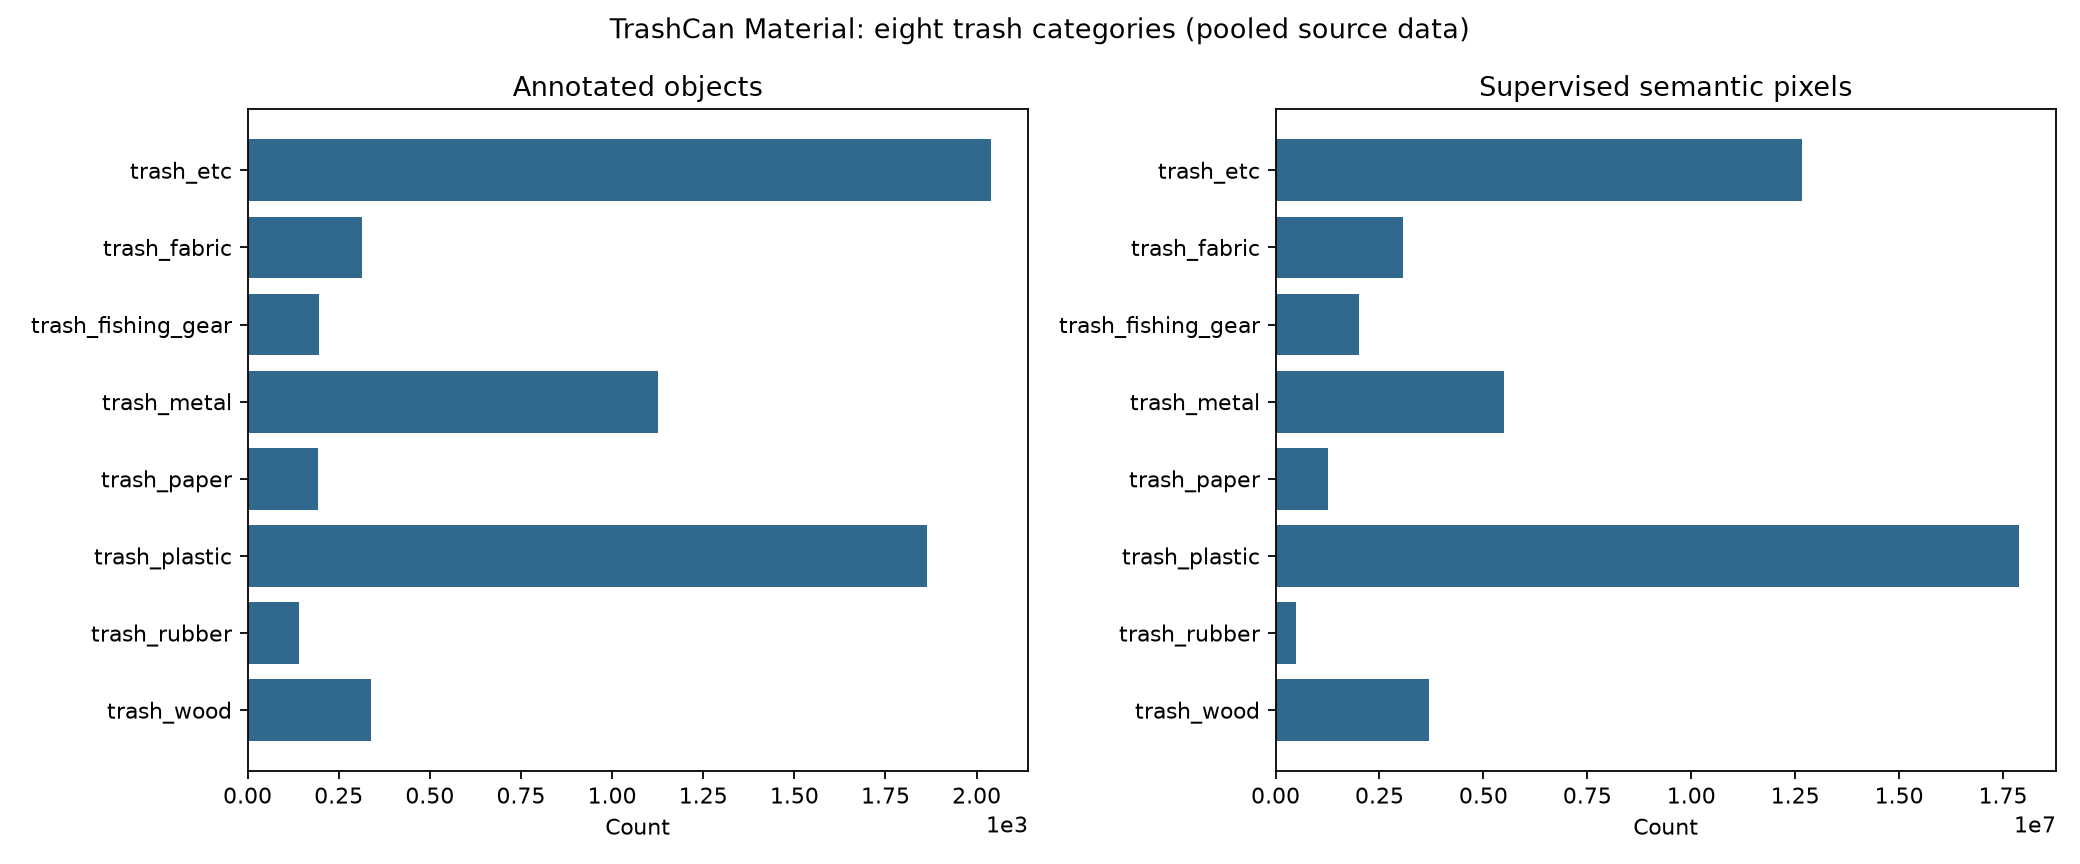
\includegraphics[width=.94\textwidth]{images/material_distribution.png}
\caption{Material-category distribution from the retained EDA.}\label{fig:distribution}
\end{figure}
\begin{figure}[H]\centering
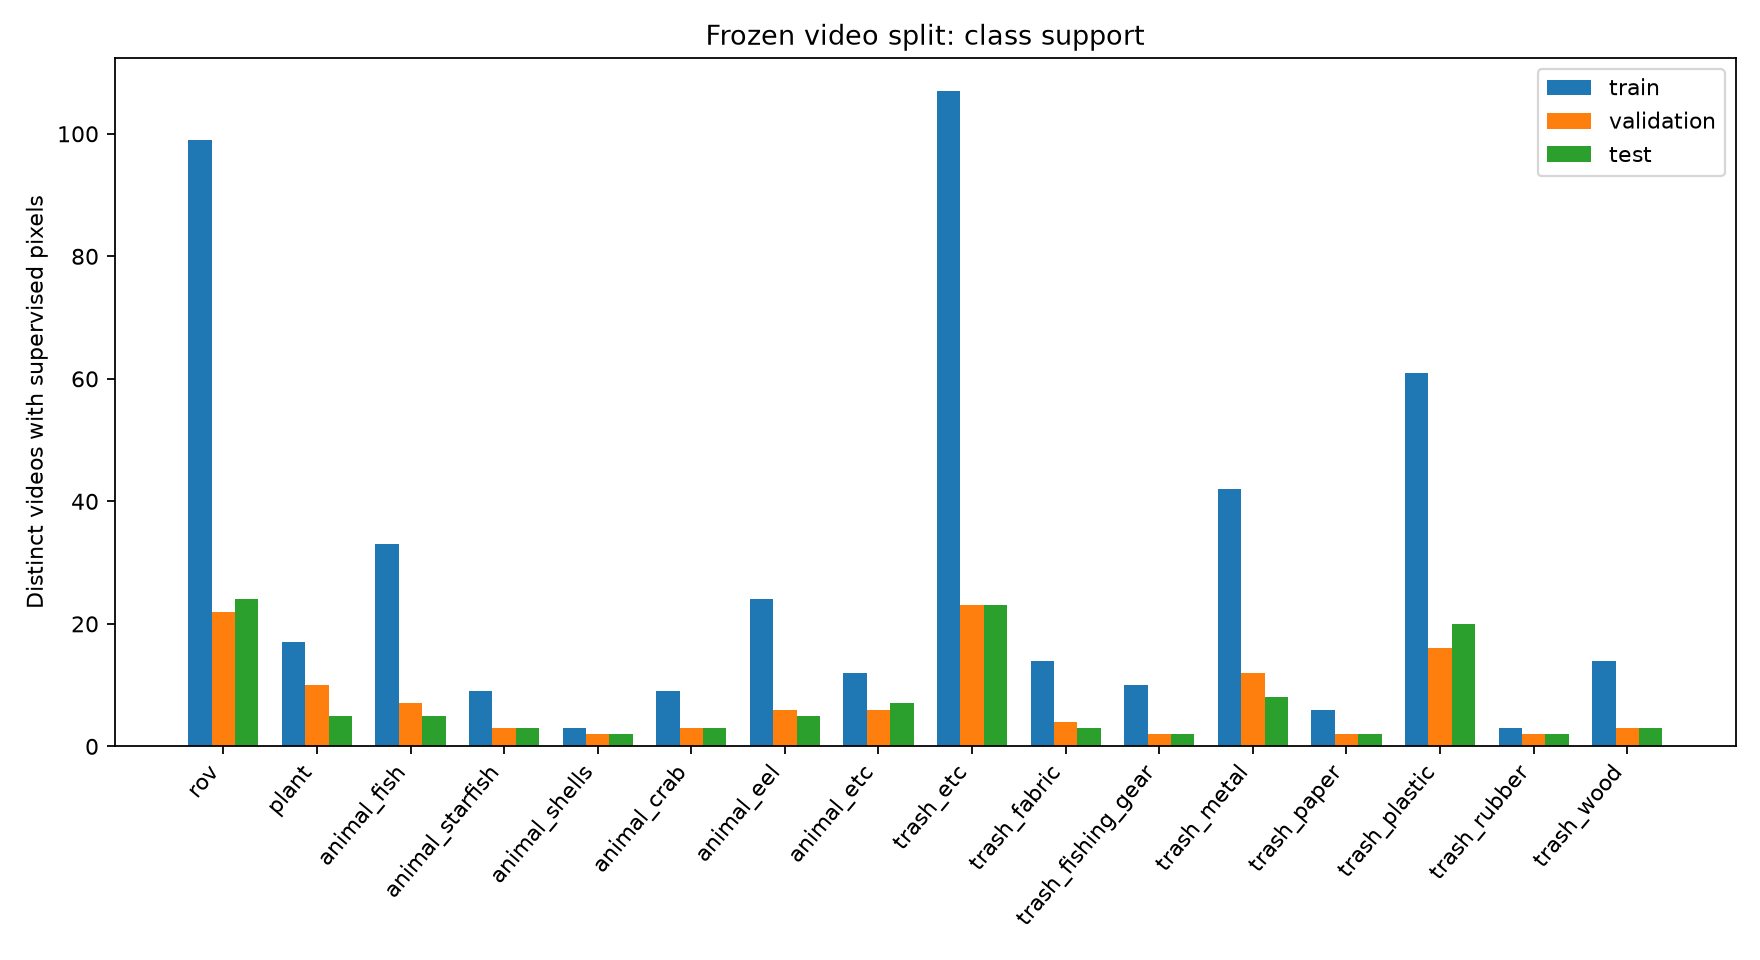
\includegraphics[width=.94\textwidth]{images/split_class_video_support.png}
\caption{Per-class video support under the fixed seed 36 split.}\label{fig:videos}
\end{figure}
The split provides class coverage in every partition while retaining rare classes; it does not remove their statistical uncertainty.

\subsection{Mask conversion, preprocessing and checks}
Polygons are rasterized on the native image canvas with Pillow 12.3.0. Same-class polygons are unioned; pixels where different foreground classes overlap receive ignore 255. Out-of-canvas regions are clipped. The EDA found no annotation that rasterized to an empty mask under this converter.

Each image is letterboxed to $512\times 512$ while preserving aspect ratio. RGB uses bilinear resizing, masks use nearest-neighbor resizing, RGB padding is black and target padding is ignore 255. The tensor is normalized with ImageNet channel means $(0.485,0.456,0.406)$ and standard deviations $(0.229,0.224,0.225)$. There is no label reduction or second image-processor resize.

The training adapter checks the published manifest digest, source annotation hashes, image dimensions, membership and native target hash. The supplied checks cover 5,057 training and 1,077 validation images. Figure~\ref{fig:qa} reproduces existing EDA annotation checks; it is not a gallery of model predictions.
At evaluation resolution, ignored pixels include the much larger letterbox padding region as well as native annotation conflicts. For example, U-Net test ignore fraction is 34.06\%; this does not mean that 34.06\% of the native annotations are conflicting.
\begin{figure}[H]\centering
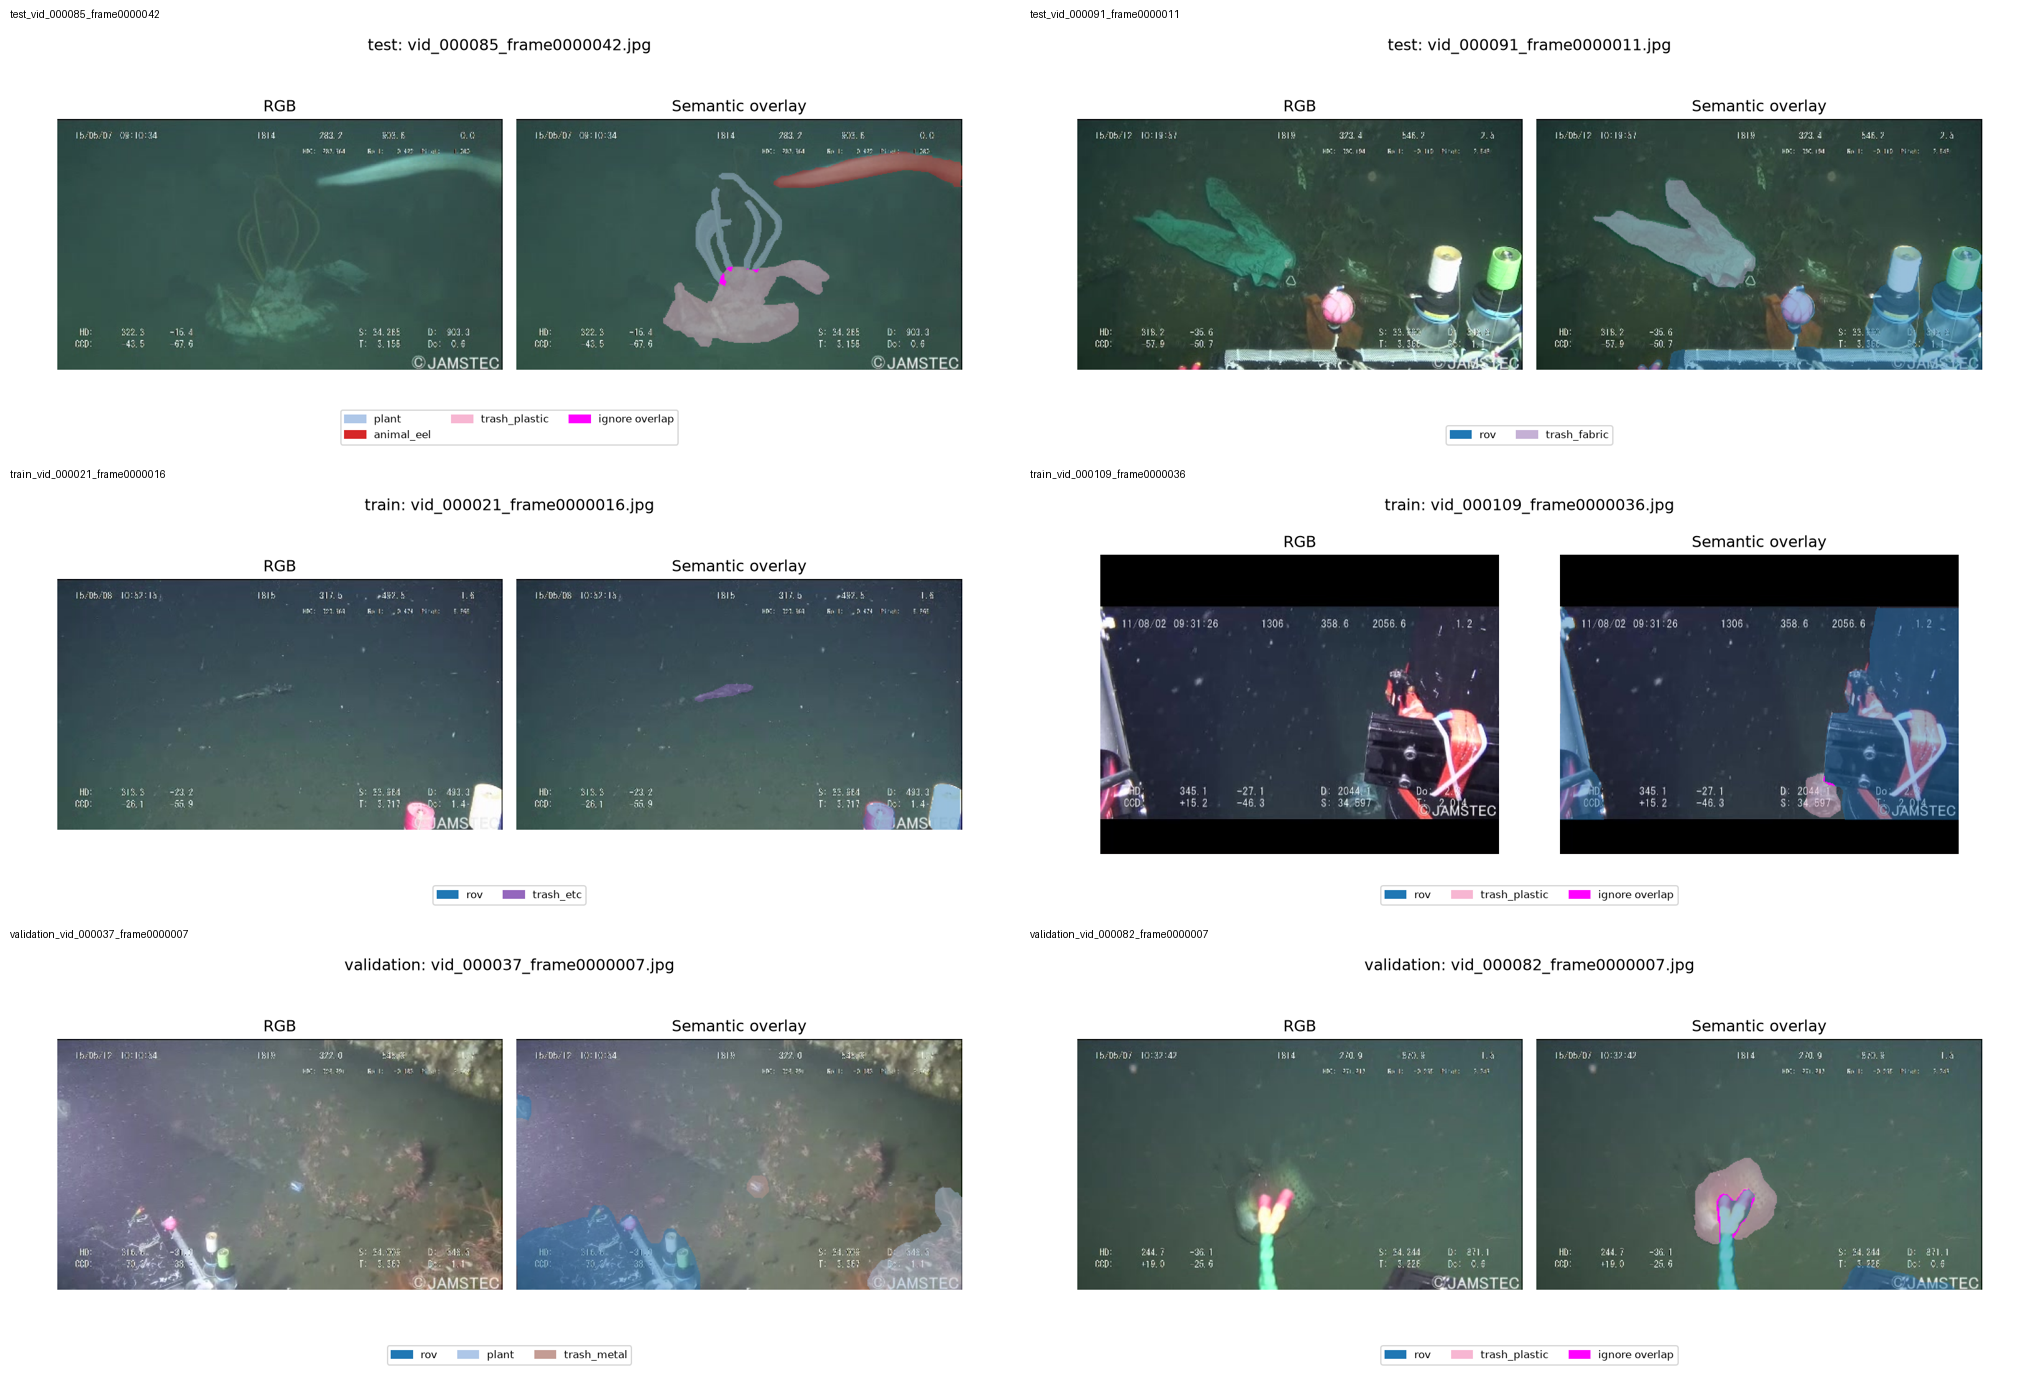
\includegraphics[width=.92\textwidth]{images/annotation_qa.png}
\caption{Six retained native annotation-QA examples, two per partition. RGB/mask overlays check conversion and alignment; they are ground truth, not inference outputs.}\label{fig:qa}
\end{figure}
